% Escreve sobre como é o formato do software e sobre modelagem paramétrica. 
Este trabalho propõe o desenvolvimento de uma plataforma computacional para o dimensionamento otimizado de pontes de madeira, empregando uma abordagem multiobjetivo baseada na norma NBR 7190 \cite{NBR7190-1:2022}. A metodologia combina a formulação estrutural segundo critérios normativos, a definição de funções objetivo e restrições, e a aplicação de uma metaheurística para obter soluções eficientes.

Foram consideradas pontes hipotéticas de madeira, submetidas a verificações de flexão, cisalhamento e flecha. O comportamento estrutural é avaliado por meio de modelos determinísticos, utilizando propriedades mecânicas características e ações de projeto estabelecidas pela norma.

O problema de dimensionamento é formulado como uma otimização multiobjetivo, cujas variáveis de decisão são as dimensões geométricas da seção transversal da viga (diâmetro, espaçamento entre longarinas, base e altura do tabuleiro). As funções objetivo, antagônicas entre si, são:
\begin{itemize}
    \item minimização da área total da viga;
    \item maximização da relação $\dfrac{\delta_{\text{total}}}{L/250}$.
\end{itemize}
A redução da área tende a aumentar as deformações, enquanto o aumento da rigidez exige mais material. Busca-se, assim, um conjunto de soluções viáveis representado por uma Fronteira de Pareto.

As restrições do problema envolvem as verificações normativas de resistência à flexão, cisalhamento e deslocamentos máximos, conforme a NBR 7190 \cite{NBR7190-1:2022}.

Para resolver o problema, utiliza-se uma metaheurística (NSGA-II) que explora o espaço de soluções de forma iterativa, avaliando populações de candidatos com base nos valores das funções objetivo e no atendimento às restrições. A abordagem permite obter a fronteira de Pareto, oferecendo ao projetista um conjunto de alternativas viáveis para a decisão.

A plataforma é implementada em \textit{Python}, com bibliotecas científicas para cálculo numérico e otimização. Os resultados são apresentados de forma gráfica e numérica, incluindo a visualização da fronteira de Pareto, possibilitando uma análise comparativa eficiente.

O fluxo metodológico adotado é composto pelas seguintes etapas:
\begin{enumerate}
    \item Definição geométrica e das cargas permanentes;
    \item Definição do trem-tipo conforme normas;
    \item Análise estrutural para obtenção de esforços e deslocamentos;
    \item Combinações de ações para estados limites último (ELU) e de serviço (ELS);
    \item Determinação das resistências de cálculo do material;
    \item Verificações estruturais; caso não atendidas, retorna-se às etapas anteriores;
    \item Aplicação do algoritmo NSGA-II para obtenção da fronteira eficiente;
    \item Seleção da solução final pelo projetista entre as soluções viáveis.
\end{enumerate}

\begin{figure}[htpb!]
    \centering
    \captionsetup{
        labelfont={bf,small}, 
        font={small},
        labelsep=endash
    }
    \caption{Fluxograma para otimização do dimensionamento de pontes de madeira.}
    \label{fig:fluxograma} 
    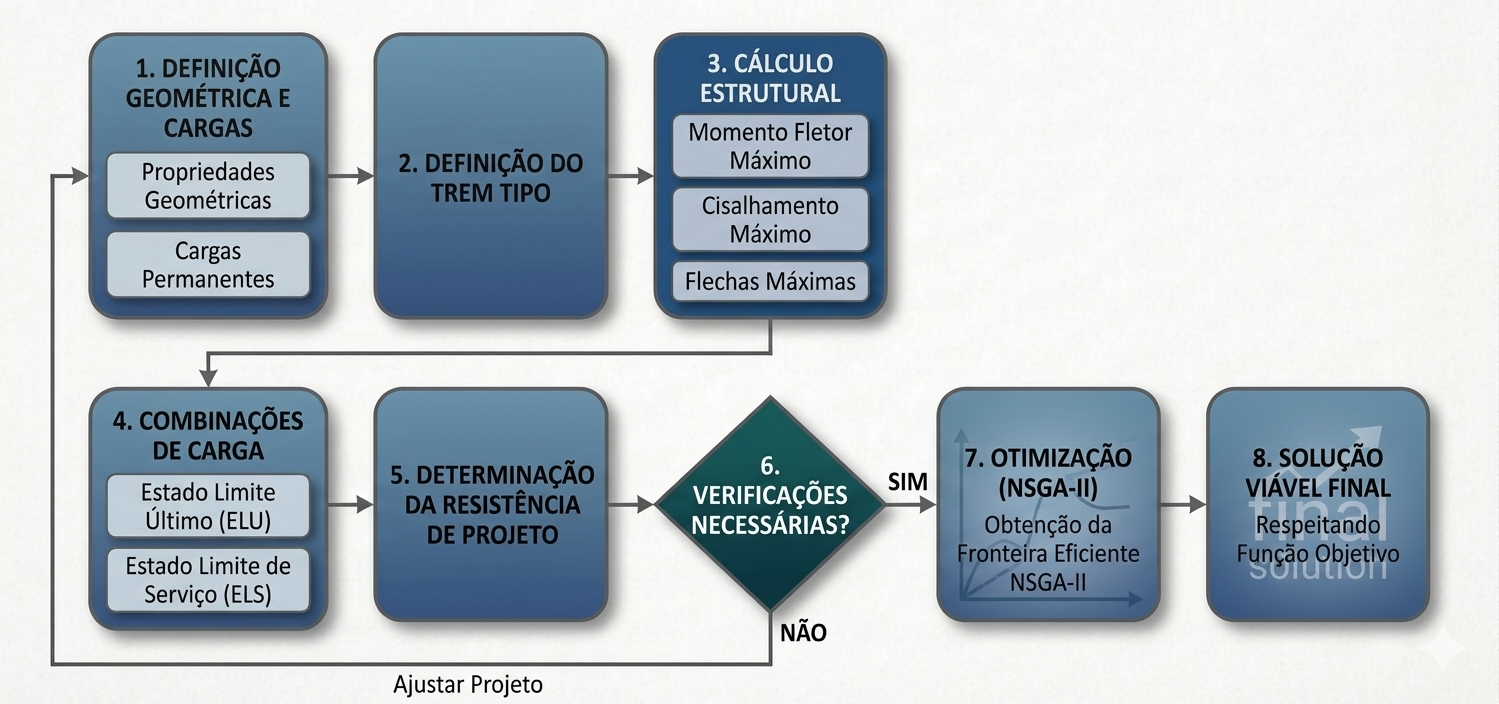
\includegraphics[width=0.8\textwidth]{imgs/fluxograma.png}
    \vspace{0.1cm}
    \par {\fontsize{11pt}{13.2pt}\selectfont \textbf{Fonte:} Autoria própria (2026).}
\end{figure}

\subsection{Dimensionamento de pontes de madeira}
% Breve intro sobre pontes de madeira (2 paragrafos no máximos). Esta ferramenta é para pontes de tal e tal jeito.


A madeira é um dos materiais mais antigos empregados na construção civil, destacando-se em pontes de pequeno e médio porte por sua elevada relação resistência-peso, durabilidade quando adequadamente tratada e baixo impacto ambiental. Em estruturas de pontes, especialmente as de madeira roliça, o material é utilizado em sua forma natural, preservando as características circulares das seções transversais e proporcionando soluções esteticamente integradas à paisagem, além de rápida execução e eficiência estrutural para vãos de até 15 metros.

O dimensionamento adequado dessas pontes exige a consideração simultânea de múltiplos critérios normativos, como os estados limites últimos e de serviço estabelecidos pela NBR 7190 \cite{NBR7190-1:2022}, além da análise de cargas permanentes e móveis (trem-tipo). A complexidade desse processo motivou o desenvolvimento de ferramentas computacionais baseadas em otimização multiobjetivo, capazes de explorar o compromisso entre a minimização do consumo de material e a maximização do desempenho estrutural, oferecendo ao projetista soluções eficientes e racionais para o projeto preliminar de pontes em madeira roliça.



\subsubsection{Levantamento de cargas}

\subsection*{Resumo das Ações e Dimensionamento de Pontes de Madeira Roliça}

O texto aborda as etapas fundamentais para a determinação dos esforços solicitantes em pontes de madeira roliça, com foco nas ações permanentes e móveis, bem como nos coeficientes de ponderação e combinações de esforços para o dimensionamento segundo as normas brasileiras NBR 8681 e NBR 7190.

\subsubsection*{Ações Permanentes}
Segundo a \textcite{NBR8681:2025}, as ações permanentes atuam continuamente ao longo da vida útil da estrutura. Em pontes de madeira roliça, incluem-se o peso próprio de elementos como longarinas, tabuleiro e rodeiros. O cálculo é realizado pela Equação~\eqref{eq:acoes_permanentes_resumo}, em função da geometria e do peso específico dos materiais.
\begin{equation}
G = \gamma \cdot A
\label{eq:acoes_permanentes_resumo}
\end{equation}
Onde:
\begin{itemize}
    \item $G$: Peso próprio (kN/m);
    \item $\gamma$: Peso específico do material (kN/m³);
    \item $A$: Área da seção transversal (m²).
\end{itemize}

\subsubsection*{Ações Móveis (Trem-Tipo)}
A carga móvel rodoviária é definida pela \textcite{nbr7188}. Os principais modelos são:
\begin{itemize}
    \item \textbf{TB-450}: Veículo-tipo com peso total de 450 kN (6 rodas de 75 kN), três eixos espaçados em 1,5 m, ocupando 18,0 m², com carga de multidão de 5 kN/m².
    \item \textbf{TB-240}: Carga mínima para estradas vicinais, com peso total de 240 kN (6 rodas de 40 kN), três eixos espaçados em 1,5 m, ocupando 18,0 m², com carga de multidão de 4 kN/m².
\end{itemize}

Para considerar os efeitos dinâmicos da passagem do veículo, aplica-se o \textbf{Coeficiente de Impacto Vertical (CIV)}, conforme as Equações \eqref{eq:CIV10_resumo} e \eqref{eq:CIVmaior_resumo}.
\begin{equation}
CIV = 1{,}35 \quad \text{para } L \leq 10{,}0 \text{ m}
\label{eq:CIV10_resumo}
\end{equation}
\begin{equation}
CIV = 1 + 1{,}06 \left( \frac{20}{LIV + 50} \right) \quad \text{para } 10{,}0 < L \leq 200{,}0 \text{ m}
\label{eq:CIVmaior_resumo}
\end{equation}
Onde $LIV$ é o comprimento característico da estrutura.





% \subsubsection{Combinações}

\subsubsection{Combinações de Ações e Verificações de Segurança}

Para a verificação da segurança e do desempenho em serviço de estruturas de madeira, torna-se necessário estabelecer critérios adequados para a combinação das ações atuantes, considerando tanto os Estados Limite Último (ELU) quanto os Estados Limite de Serviço (ELS). A NBR 7190 \textcite{NBR7190-1:2022} define procedimentos específicos para essa finalidade, levando em conta as particularidades do material madeira, como a variabilidade de suas propriedades e seu comportamento reológico diferenciado, notadamente a deformação progressiva ao longo do tempo.

\subsection{Coeficientes de Ponderação das Ações Permanentes}

Previamente à definição das combinações de ações, é necessário conhecer os esforços solicitantes característicos atuantes na estrutura. A NBR 7190 \parencite{NBR7190-1:2022} estabelece os coeficientes de ponderação $\gamma_{g}$ a serem aplicados às ações permanentes, apresentando três conjuntos de valores possíveis, cuja escolha fica a critério do projetista em função do nível de segurança pretendido, conforme discriminado a seguir:

\begin{enumerate}[label=\alph*)]
    \item $\gamma_{g} = 1,3;\ \gamma_{g} = 1,2;\ \gamma_{g} = 1,15;$ para elementos estruturais de madeira em geral;
    \item $\gamma_{g} = 1,25;\ \gamma_{g} = 1,15;\ \gamma_{g} = 1,10;$ para elementos estruturais industrializados de madeira;
\end{enumerate}

\subsection{Combinações para o Estado Limite Último (ELU)}

Para a verificação da segurança estrutural no domínio do Estado Limite Último (ELU), a NBR 7190 \parencite{NBR7190-1:2022} remete à NBR 8681 \parencite{NBR8681:2025}. Adota-se, nesse contexto, a combinação última normal, que contempla situações com probabilidade de ocorrência suficientemente elevada durante a vida útil da estrutura. A expressão geral para essa combinação é apresentada na Equação \eqref{eq:2.01}.

\begin{equation}
F_d = \sum_{i=1}^{m} \gamma_{gi}\, F_{Gi,k}
      + \gamma_{q1}\, F_{Q1,k}
      + \sum_{j=2}^{n} \gamma_{qj}\, F_{Qj,k}\, \psi_{0j}
       \label{eq:2.01}
\end{equation}

Onde:

\begin{tabular}{ll}
$F_d$            & valor de cálculo da ação combinada; \\
$\gamma_{gi}$    & coeficiente de majoração das ações permanentes; \\
$F_{G i,k}$      & valor característico das ações permanentes; \\
$\gamma_{q1}$    & coeficiente de majoração da ação variável principal; \\
$F_{Q1,k}$       & valor característico da ação variável principal; \\
$\gamma_{qj}$    & coeficiente de majoração das ações variáveis secundárias; \\
$\psi_{0j}$      & fator de combinação das ações variáveis secundárias; \\
$F_{Qj,k}$       & valor característico das ações variáveis secundárias; \\
$m$, $n$         & números de ações permanentes e de ações variáveis consideradas.
\end{tabular}

No âmbito do presente estudo, adotou-se a combinação última normal em conformidade com a NBR 7190 \parencite{NBR7190-1:2022}. Para o dimensionamento da longarina de madeira, considerou-se o trem-tipo como ação variável principal. Nesse contexto, aplicou-se a redução prevista na norma ao valor característico dessa ação, resultando na expressão apresentada na Equação \eqref{eq:2.09}. Tal redução é aplicada exclusivamente às verificações dos elementos estruturais de madeira.

\begin{equation}
      F_d = \sum_{i=1}^{m} \gamma_{gi}\, F_{Gi,k}
      + \gamma_{qw}\, 0{,}75\, F_{Qw,k}
      + \gamma_{q2}\, \psi_{0,q2}\, F_{Q2,k}
      \label{eq:2.09}
\end{equation}

Onde:

\begin{tabular}{ll}
$\gamma_{qw}$    & coeficiente de majoração da ação do vento; \\
$\gamma_{q2}$    & coeficiente de majoração da ação variável secundária; \\
$\psi_{0,q2}$    & fator de combinação da ação variável secundária; \\
$F_{Qw,k}$       & valor característico da ação do vento; \\
$F_{Q2,k}$       & valor característico da ação variável secundária.
\end{tabular}

\subsection{Combinações para o Estado Limite de Serviço (ELS)}

Objetivando garantir condições adequadas de utilização, durabilidade e conforto aos usuários, as estruturas de madeira devem ser verificadas quanto aos Estados Limite de Serviço (ELS). Essas verificações visam evitar deformações ou deslocamentos excessivos que possam comprometer a funcionalidade da construção, causar danos estéticos ou induzir vibrações indesejáveis. A NBR 7190 \parencite{NBR7190-1:2022} estabelece, para tanto, critérios associados à deformabilidade da estrutura, considerando dois cenários distintos: os deslocamentos instantâneos ($\delta_{\mathrm{inst}}$) e os deslocamentos finais ou efetivos ($\delta_{\mathrm{fin}}$).

A madeira distingue-se de outros materiais estruturais por apresentar deformação significativa ao longo do tempo sob carregamento constante, fenômeno conhecido como fluência. Em função desse comportamento reológico, as verificações de serviço devem considerar separadamente os efeitos imediatos e os efeitos diferidos.

Para a avaliação das flechas instantâneas ($\delta_{\mathrm{inst}}$), que correspondem às deformações imediatas da estrutura desconsiderando os efeitos da fluência, adota-se a combinação rara de serviço, conforme estabelecido pela NBR 8681 \parencite{NBR8681:2025}. O cálculo desses deslocamentos é realizado conforme a Equação \eqref{eq:flecha_inst}.

\begin{equation}
\delta_{\mathrm{inst}} =
\sum_{i=1}^{m} \delta_{\mathrm{inst},G_i,k}
+ \delta_{\mathrm{inst},Q_1,k}
+ \sum_{j=2}^{n} \delta_{\mathrm{inst},Q_j,k} \cdot \psi_{1,j}
\label{eq:flecha_inst}
\end{equation}

Onde:

\begin{tabular}{ll}
$\delta_{\mathrm{inst},G_i,k}$ & flechas instantâneas decorrentes das ações permanentes; \\
$\delta_{\mathrm{inst},Q_1,k}$ & flecha instantânea associada à ação variável principal; \\
$\delta_{\mathrm{inst},Q_j,k}$ & flechas instantâneas decorrentes das ações variáveis secundárias; \\
$\psi_{1,j}$ & fator de redução correspondente à combinação frequente.
\end{tabular}

Para a avaliação das flechas finais ($\delta_{\mathrm{fin}}$), que incorporam os efeitos da fluência da madeira, a NBR 7190 \parencite{NBR7190-1:2022} prescreve a utilização da combinação quase permanente de ações, conforme a Equação \eqref{eq:flecha_fin}.

\begin{equation}
\delta_{\mathrm{fin}} =
\sum_{i=1}^{m} \delta_{\mathrm{fin},G_i,k}
+ \sum_{j=1}^{n} \delta_{\mathrm{fin},Q_j,k}
\label{eq:flecha_fin}
\end{equation}

Onde:

\begin{tabular}{ll}
$\delta_{\mathrm{fin},G_i,k}$ & flechas finais associadas às ações permanentes; \\
$\delta_{\mathrm{fin},Q_j,k}$ & flechas finais associadas às ações variáveis, calculadas conforme as Equações \eqref{eq:flecha_fin_G} e \eqref{eq:flecha_fin_Q}.
\end{tabular}

As parcelas de flecha final decorrentes das ações permanentes e variáveis são obtidas, respectivamente, por meio das expressões:

\begin{equation}
\delta_{\mathrm{fin},G_i,k}
=
\delta_{\mathrm{inst},G_i,k}
+ \delta_{\mathrm{creep}}
=
\delta_{\mathrm{inst},G_i,k} \cdot (1 + \varphi)
\label{eq:flecha_fin_G}
\end{equation}

\begin{equation}
\delta_{\mathrm{fin},Q_j,k}
=
\delta_{\mathrm{inst},Q_j,k}
+ \delta_{\mathrm{creep}}
=
\delta_{\mathrm{inst},Q_j,k} \cdot \psi_{2} \cdot (1 + \varphi)
\label{eq:flecha_fin_Q}
\end{equation}

Onde:

\begin{tabular}{ll}
$\delta_{\mathrm{creep}}$ & parcela da flecha associada aos efeitos da fluência da madeira; \\
$\varphi$ & coeficiente de fluência da madeira, definido conforme o Quadro \ref{qua:fluencia}; \\
$\psi_{2}$ & fator de redução correspondente à combinação quase permanente.
\end{tabular}

O coeficiente de fluência ($\varphi$) é determinado em função do tipo de material empregado e da classe de umidade à qual a estrutura está exposta. Observa-se que classes de umidade mais elevadas implicam maiores deformações diferidas, conforme os valores apresentados no Quadro \ref{qua:fluencia}.

\clearpage
\begin{quadro}[htpb!]
    \centering
    % Define o nome como Quadro para este elemento específico
    \renewcommand{\tablename}{Quadro}
    
    % Configura o negrito e o tamanho 11pt para a Legenda (no topo)
    \captionsetup{
        labelfont={bf,small}, 
        font={small},
        labelsep=endash
    }
    \caption{Coeficiente de fluência ($\varphi$).}
    \label{qua:fluencia}

    % Definição do quadro (formato fechado) com tamanho 11pt
    \fontsize{11pt}{13.2pt}\selectfont
    \begin{tabular}{|>{\centering\arraybackslash}m{6.0cm}|>{\centering\arraybackslash}m{2.5cm}|>{\centering\arraybackslash}m{2.5cm}|>{\centering\arraybackslash}m{2.5cm}|}
        \hline
        \textbf{Materiais} & \multicolumn{3}{c|}{\textbf{Classe de umidade}} \\ \cline{2-4} 
         & \textbf{(1)} & \textbf{(2 e 3)} & \textbf{(4)} \\ \hline
        Madeira serrada, MLC, MLCC, LVL e roliça & 0,6 & 0,8 & 2,0\textsuperscript{a} \\ \hline
        Compensado estrutural & 0,8 & 1,0 & 2,5 \\ \hline
        OSB estrutural & 1,5 & 2,25 & -- \\ \hline
    \end{tabular}

    % Notas e Fonte com tamanho 11pt
    \vspace{0.1cm}
    \par {\fontsize{11pt}{13.2pt}\selectfont \textsuperscript{a} Não é permitido o uso de MLCC para a classe de umidade 4.}
    
    \par {\fontsize{11pt}{13.2pt}\selectfont \textbf{Fonte:} Adaptado da NBR 7190 \parencite{NBR7190-1:2022}.}
\end{quadro}

\subsubsection{Propriedades da madeira}

A determinação das propriedades geométricas da seção transversal constitui uma etapa fundamental na análise e no dimensionamento de elementos estruturais, uma vez que essas propriedades influenciam diretamente a resistência, a rigidez e a estabilidade da estrutura. Parâmetros como área, momento de inércia, módulo resistente e raio de giração são essenciais para a verificação dos estados limites últimos e de serviço, conforme os critérios estabelecidos pela NBR 7190 \cite{NBR7190-1:2022}.

Para o caso de seções transversais circulares maciças, a área (m²) pode ser obtida conforme a Equação~\eqref{eq:1}.

\begin{equation}
A = \frac{\pi d^2}{4}
\label{eq:1}
\end{equation}

Onde, \(d\) é o diâmetro da seção transversal (m).

Por sua vez, para seções transversais de geometria retangular, a área (m²) é determinada pela Equação~\eqref{eq:2}.

\begin{equation}
A = b \cdot h
\label{eq:2}
\end{equation}

Onde, \(b\) corresponde à largura (m) e \(h\) à sua altura (m).

Os momentos de inércia em relação aos eixos principais ($m^4$) caracterizam a distribuição da área da seção transversal e são determinantes para a avaliação da rigidez à flexão dos elementos estruturais. Esses parâmetros dependem diretamente da geometria da seção analisada.

Para seções transversais circulares maciças, em razão da simetria geométrica, os momentos de inércia ($m^4$) em relação aos eixos principais \(x\) e \(y\) são idênticos, sendo expressos pela Equação~\eqref{eq:3}.

\begin{equation}
I_x = I_y = \frac{\pi d^4}{64}
\label{eq:3}
\end{equation}

Onde, \(d\) representa o diâmetro da seção (m).

Por sua vez, para seções transversais de geometria retangular, como o tabuleiro, os momentos de inércia ($m^4$) em relação aos eixos principais são distintos e definidos pelas Equações \eqref{eq:4} e \eqref{eq:5}.

\begin{equation}
I_x = \frac{b h^3}{12}
\label{eq:4}
\end{equation}

\begin{equation}
I_y = \frac{h b^3}{12}
\label{eq:5}
\end{equation}

Onde, \(b\) corresponde à largura (m)  e \(h\) à sua altura (m).

O módulo resistente (m³) está associado à capacidade da seção transversal em resistir aos momentos fletores máximos, sendo definido como a razão entre o momento de inércia e a distância da fibra mais afastada ao eixo neutro. Para seções circulares, o módulo resistente é o mesmo em ambos os eixos principais e é dado pela Equação~\eqref{eq:6}.

\begin{equation}
W_x = W_y = \frac{I_x}{d/2}
\label{eq:6}
\end{equation}

Já para seções retangulares, os módulos resistentes (m³) em relação aos eixos principais são definidos pelas Equações \eqref{eq:7} e \eqref{eq:8}.

\begin{equation}
W_x = \frac{I_x}{h/2}
\label{eq:7}
\end{equation}

\begin{equation}
W_y = \frac{I_y}{b/2}
\label{eq:8}
\end{equation}

Outro parâmetro relevante é o raio de giração (m), amplamente utilizado nas verificações de estabilidade estrutural, como a análise de flambagem. O raio de giração relaciona o momento de inércia com a área da seção transversal. Para seções circulares e retangulares, os raios de giração são expressos pelas Equações \eqref{eq:9} e \eqref{eq:10}.

\begin{equation}
r_x = \sqrt{\frac{I_x}{A}}
\label{eq:9}
\end{equation}

\begin{equation}
r_y = \sqrt{\frac{I_y}{A}}
\label{eq:10}
\end{equation}

Dessa forma, a determinação das propriedades geométricas das seções transversais circulares e retangulares fornece a base necessária para a realização das verificações estruturais, assegurando coerência entre a modelagem geométrica adotada e os critérios normativos aplicáveis.

reescreva com outras palavras, mantenha no formado de latex 

\subsubsection{Dimensionamento à flexão}

A NBR 7190 \parencite{NBR7190-1:2022} exige que a verificação da flexão simples em peças estruturais de madeira considere a possibilidade de flexão reta ou flexão oblíqua, conforme a orientação do carregamento em relação aos eixos principais de inércia da seção transversal.

No caso da flexão reta, o momento fletor atua em torno de apenas um eixo principal, gerando uma distribuição linear das tensões normais. A verificação é feita comparando-se a tensão de flexão de cálculo com a resistência de cálculo ao momento fletor, conforme apresentado na Equação~\eqref{eq:flexao_reta}.

\begin{equation}
\frac{\sigma_{Mx,d}}{f_{m,d}} = \frac{M_d}{W \, f_{m,d}} \leq 1
\label{eq:flexao_reta}
\end{equation}

Onde:

\begin{tabular}{ll}
$\sigma_{Mx,d}$ & Tensão atuante de cálculo referente à flexão em torno do eixo $x$ (kPa);\\
$f_{m,d}$ & Resistência de cálculo à flexão da madeira (kPa);\\
$M_d$ & Momento fletor solicitante de cálculo (kN.m);\\
$W_x$ & Módulo de resistência elástico da seção em relação ao eixo $x$ ($m^3$);\\
\end{tabular}

\subsection{Método de otimização multiobjetivo}

O projeto da ponte de madeira é integrado a uma estrutura de otimização multiobjetivo visando apoiar uma etapa racional e orientada ao desempenho do dimensionamento estrutural. A tarefa de otimização é formulada como um problema de otimização multiobjetivo e resolvida por meio do Algoritmo Genético de Ordenação Não Dominada II (NSGA-II), sendo adequado para problemas não lineares, com restrições e objetivos conflitantes.

Um problema de otimização multiobjetivo envolve a minimização e/ou maximização simultânea de múltiplas funções objetivo, sujeitas a um conjunto de restrições que definem a viabilidade das soluções candidatas. Diferentemente da otimização monoobjetivo ele não conduz a uma única solução ótima, alternativamente, resulta em um conjunto de soluções ótimas de Pareto, cada uma representando um caso distinto entre critérios de desempenho concorrentes.

A formulação matemática geral de um problema de otimização multiobjetivo pode ser expressa conforme a Equação~\eqref{eq:mop}.

\begin{equation}
\begin{cases} 
f_m(\mathbf{x}), & m = 1,2,\ldots,M; \\ 
g_j(\mathbf{x}) \leq 0, & j = 1,2,\ldots,J; \\ 
h_k(\mathbf{x}) = 0, & k = 1,2,\ldots,K; \\ 
x_i^{(L)} \leq x_i \leq x_i^{(U)}, & i = 1,2,\ldots,n.
\end{cases}
\label{eq:mop}
\end{equation}

Nesta formulação, o vetor de funções objetivo é definido segundo a Equação~\eqref{eq:fx}.

\begin{equation}
f(\mathbf{x}) = \left(f_1(\mathbf{x}), f_2(\mathbf{x}), \ldots, f_M(\mathbf{x})\right)^T
\label{eq:fx}
\end{equation}

Onde, $\mathbf{x} = (x_1, x_2, \ldots, x_n)^T$ representa o vetor $n$-dimensional de variáveis de projeto. 

O espaço de projeto viável é restringido por restrições de desigualdade $g_j(\mathbf{x})$, restrições de igualdade $h_k(\mathbf{x})$ e restrições de domínio definidas pelos limites inferior e superior $x_i^{(L)}$ e $x_i^{(U)}$, que em conjunto definem o domínio admissível $(D)$ \parencite{DEB2009}.

Objetivos inicialmente formulados como problemas de maximização são convertidos em problemas equivalentes de minimização por meio da multiplicação das respectivas funções objetivo por $-1$, garantindo uma estrutura de otimização unificada e consistente.

A Figura~\ref{fig:pareto} ilustra o espaço de soluções de um problema biobjetivo, destacando a diversidade de soluções viáveis e o conceito de dominância de Pareto que caracteriza a otimização multiobjetivo.

\begin{figure}[htpb!]
    \centering
    \captionsetup{
        labelfont={bf,small}, 
        font={small},
        labelsep=endash
    }
    \caption{Possíveis soluções de um problema de otimização multiobjetivo.}
    \label{fig:pareto} 
    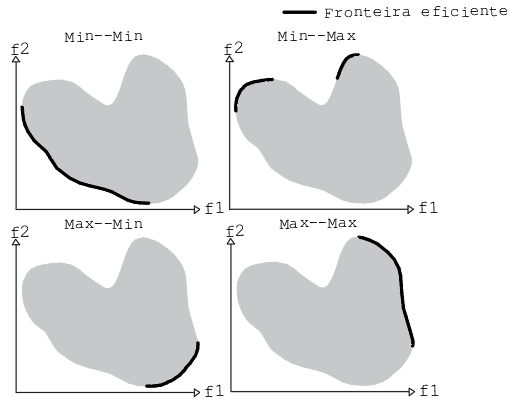
\includegraphics[width=0.6\textwidth]{imgs/z_types_frontier.png}
    \vspace{0.1cm}
    \par {\fontsize{11pt}{13.2pt}\selectfont \textbf{Fonte:} {\textcite{DEB2009}.}
 \end{figure}


 
 \subsection{Algoritmo Genético de Ordenação Não Dominada II (NSGA-II)}

 O problema de otimização multiobjetivo é resolvido utilizando o Algoritmo Genético de Ordenação Não Dominada II (NSGA-II), um algoritmo evolutivo desenvolvido especificamente para aproximar o conjunto ótimo de Pareto em problemas que envolvem objetivos conflitantes \parencite{DEB2009}. Diferentemente de abordagens baseadas em escalarização, o NSGA-II preserva a natureza multiobjetivo do problema e busca um conjunto diverso de soluções não dominadas.

Seja $f(\mathbf{x}) = \left(f_1(\mathbf{x}), f_2(\mathbf{x}), \ldots, f_M(\mathbf{x})\right)^T$ o vetor de funções objetivo. Dadas duas soluções candidatas $\mathbf{x}^a$ e $\mathbf{x}^b$, diz-se que $\mathbf{x}^a$ \textit{domina no sentido de Pareto} $\mathbf{x}^b$, denotado por $\mathbf{x}^a \prec \mathbf{x}^b$, se atende as condições da Equação \eqref{eq:333}.

\begin{equation}
\forall m \in \{1,\ldots,M\}, \; f_m(\mathbf{x}^a) \leq f_m(\mathbf{x}^b)
\quad \text{e} \quad
\exists m \; : \; f_m(\mathbf{x}^a) < f_m(\mathbf{x}^b)
\label{eq:333}
\end{equation}

A cada geração, a população é ordenada em frentes sucessivas não dominadas $\mathcal{F}_1, \mathcal{F}_2, \ldots$, sendo $\mathcal{F}_1$ o conjunto de soluções não dominadas, representando a aproximação atual da fronteira de Pareto. A seleção dos indivíduos é baseada tanto na hierarquia de Pareto quanto na diversidade das soluções.

Para preservar a diversidade ao longo da fronteira de Pareto, o NSGA-II emprega a métrica denominada distância de aglomeração (\textit{crowding distance}). Para uma solução $\mathbf{x}_i$ pertencente a uma determinada frente, a distância de aglomeração $d_i$ é calculada conforme a Equação~\eqref{eq:diversidade}.

\begin{equation}
d_i = \sum_{m=1}^{M}
\frac{f_m(\mathbf{x}_{i+1}) - f_m(\mathbf{x}_{i-1})}
{f_m^{\max} - f_m^{\min}}
\label{eq:diversidade}
\end{equation}

Onde, $f_m^{\max}$ e $f_m^{\min}$ representam, respectivamente, os valores máximo e mínimo da $m$-ésima função objetivo dentro da mesma frente. Soluções localizadas em regiões menos densas do espaço de objetivos são preferidas, promovendo uma distribuição uniforme da fronteira eficiente.

Uma estratégia elitista é adotada por meio da combinação das populações parental e descendente, sendo os melhores indivíduos selecionados com base no nível de Pareto e na distância de aglomeração. O resultado final do processo de otimização é uma aproximação da fronteira eficiente de Pareto, representando um conjunto de alternativas de projeto viáveis, nas quais a melhoria de um objetivo implica necessariamente a degradação de pelo menos outro.

\subsection{Tratamento das restrições}

O tratamento das restrições a base de otimização multiobjetivo propõe uma abordagem baseada em viabilidade, conforme implementado na Biblioteca de otimização \texttt{pymoo} \parencite{blank2020}. Dessa forma, o problema de otimização multiobjetivo com restrições é definido por um conjunto de restrições de desigualdade e igualdade, expressas, respectivamente, segundo as Equações \eqref{eq:g} e \eqref{eq:h}.

\begin{equation}
g_j(\mathbf{x}) \leq 0, \quad j = 1,2,\ldots,J
\label{eq:g}
\end{equation}

e

\begin{equation}
h_k(\mathbf{x}) = 0, \quad k = 1,2,\ldots,K
\label{eq:h}
\end{equation}

As restrições de igualdade são internamente transformadas em restrições de desigualdade por meio da introdução de uma tolerância numérica $\varepsilon$, conforme a expressão \eqref{eq:hk}.

\begin{equation}
|h_k(\mathbf{x})| - \varepsilon \leq 0
\label{eq:hk}
\end{equation}

Para cada solução candidata $\mathbf{x}$, é calculada uma medida agregada de violação das restrições $\mathrm{CV}(\mathbf{x})$, segundo a Equação~\eqref{eq:sum}.

\begin{equation}
\mathrm{CV}(\mathbf{x}) =
\sum_{j=1}^{J} \max\left(0, g_j(\mathbf{x})\right)
+
\sum_{k=1}^{K} \max\left(0, |h_k(\mathbf{x})| - \varepsilon \right)
\label{eq:sum}
\end{equation}

Uma solução é considerada viável se $\mathrm{CV}(\mathbf{x}) = 0$, sendo considerada inviável caso contrário. Durante o processo evolutivo, a comparação e seleção das soluções seguem as regras de viabilidade originalmente propostas por \textcite{DEB2009}. De acordo com essas regras, soluções viáveis sempre dominam soluções inviáveis; entre soluções viáveis, aplica-se a dominância de Pareto; e, entre soluções inviáveis, a ordenação é baseada no grau total de violação das restrições \parencite{DEB2009}.

Essa estratégia orientada pela viabilidade permite que o processo de otimização convirja de forma consistente e numericamente robusta para a fronteira de Pareto viável, sem a necessidade de funções de penalização ou reformulação das funções objetivo, sendo particularmente adequada para problemas de otimização estrutural com múltiplos objetivos e restrições rigorosas \parencite{blank2020}.

% This section outlines the framework development process and demonstrates its application through parametric structural design. The methodology is organized as follows: \textbf{a) Structural Modeling Approach}, presenting the beam conceptualization and internal load analysis for the adopted simply supported beam configuration; \textbf{b) Design of timber elements}, detailing the verification equations for bending moment, shear, and displacement compliance with NBR 7190 standards; and \textbf{c) Optimization Process}, describing the objective functions and constraint formulations. Figure~\ref{fig:z_flux_data_framework} illustrates the overall framework workflow.

% \subsection{Illustrative examples}
% Esta seção descreve os locais de instalação das pontes que serão objeto de projeto neste software. As estruturas em questão, situadas no município de Ipameri, encontram-se em estado precário, demandando intervenção urgente.
% Com o objetivo de subsidiar a análise estrutural e a caracterização espacial para os futuros projetos, foram realizadas visitas técnicas de inspeção a três pontes na região. Os dados e observações coletados in loco são detalhados a seguir na tabela \ref{tab:classes_resistencia}.


% % Tabela
% % Local, latitude, longitude, altitude, vão da pista, vão livre, Rodovia, carga permanente (se tem capa asfáltica) kN/m²

% \renewcommand{\arraystretch}{2}
% \begin{table}[htbp]
% \captionsetup{position=top}
% \centering
% \caption{Características Técnicas e Georreferenciamento das Pontes Inspecionadas em Ipameri.}
% \label{tab:classes_resistencia}
% \footnotesize
% \begin{tabular}{>{\centering\arraybackslash}p{2 cm} 
%                 >{\centering\arraybackslash}p{4.5 cm}
%                 >{\centering\arraybackslash}p{4.5 cm}
%                 >{\centering\arraybackslash}p{4.5 cm}}
% \hline
% \textbf{Pontes} & \textbf{ Rio do Braço} & \textbf{Três Bocas} & \textbf{ Mascarenhas de Morais} \\\hline

% \raisebox{6\height}{\textbf{Ilustração}}
% & 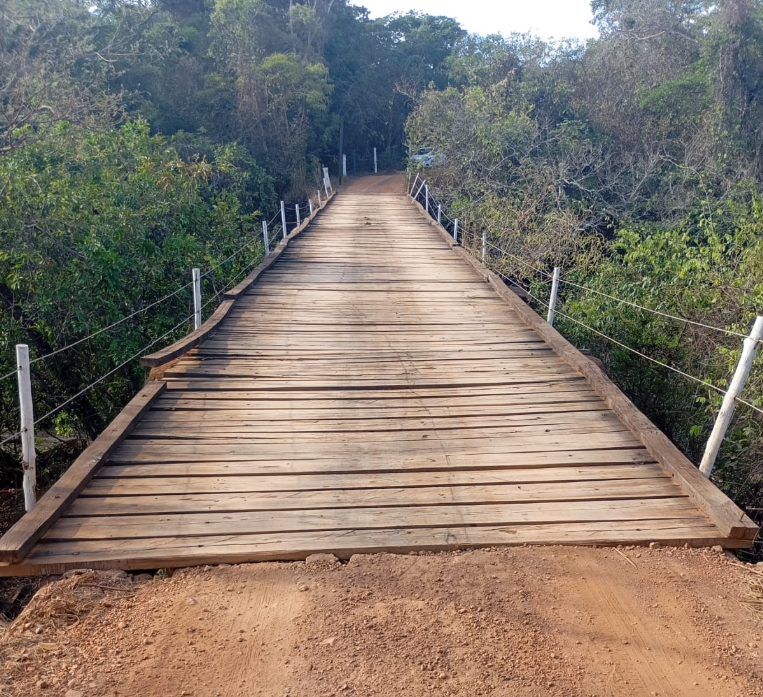
\includegraphics[width=3.3cm]{imgs/Rio do Braço.png} 
% & 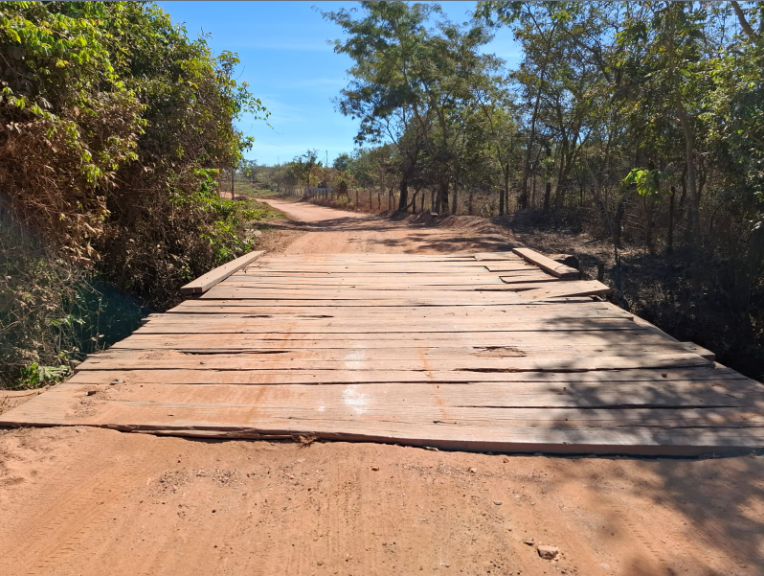
\includegraphics[width=4cm]{imgs/Tres bocas.png}
% & 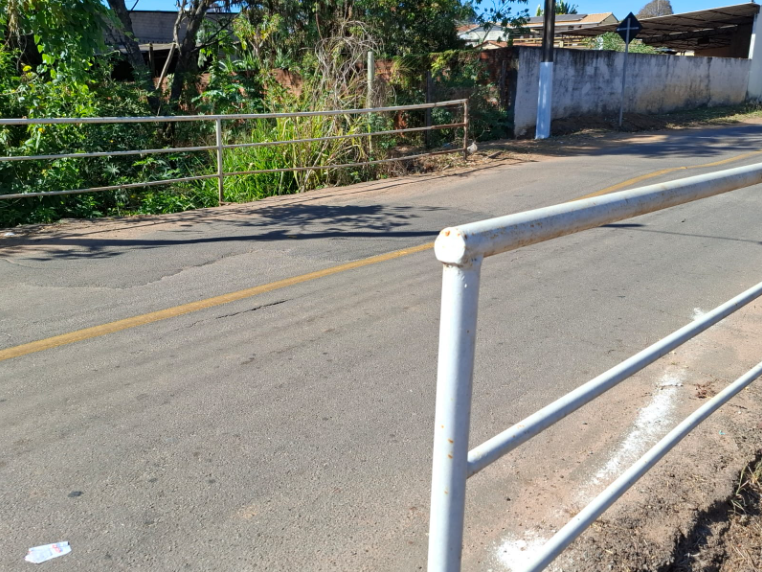
\includegraphics[width=4cm]{imgs/Mascarenha de morais.png} \\%\hline

% \textbf{Localização} & Estra. Prainha & Estra. Acesso ao Ribe. Três Bocas & Rua Masc. de Morais \\%\hline

% \textbf{Latitude} & -17°45’03.5" & -17°75’43.71" & -17°43’53.5" \\%\hline

% \textbf{Longitude} & -48°09’55.2" & -48°18’43.90" & 48°09’54.9" \\%\hline

% \textbf{Altitude} & 668 m & 682 m & 739 m \\%\hline

% \textbf{Comprimento} & 13,4 m & 6,4 m & 7 m \\%\hline

% \textbf{Largura } & 3,5 m & 3,5 m & 7 m \\%\hline

% \textbf{Tipo Longarinas} & Mad. Roliça & Mad. Roliça & Mad. Roliça \\%\hline

% \textbf{Massa Asfáltica} & Não Aplica & Não Aplica & 0.69 kN/m2 \\%\hline

% \textbf{Sist. Estrutural} & Biapoiado & Biapoiado & Biapoiado \\
% \hline
% \end{tabular}
% %\small Fonte: Autoria Propriá.
% \end{table}

% A tabela evidencia a heterogeneidade das estruturas inspecionadas, com variações significativas em localização geográfica, altitude e dimensão do vão. A ausência do dado de carga permanente para duas das pontes destaca uma possível limitação nos dados disponíveis ou uma diferença no método de inspeção aplicado em cada caso, informação crucial para as próximas etapas de análise estrutural.



% \begin{figure}[htbp!]
%     \centering
%     \includegraphics[width=0.5\textwidth]{z_flux_data_framework.png}
%     \caption{User interaction flowchart with the structural optimization framework.}
%     \label{fig:z_flux_data_framework}
% \end{figure}

% \subsection{Structural Modeling Approach}
% The simply supported beam configuration was adopted as the primary structural scheme due to its prevalence in practical applications. Internal force distributions were derived through classical solid mechanics formulations. Table~\ref{fig:exemplo} enumerates the complete internal load regimes and associated displacement fields under both permanent (dead) and load train conditions.

% As Equações xxx a xx rperesentam os valores máximos de mommentos

% \begin{table}[htbp!]
% \centering
% \caption{Loads and internal loads for girders.}
% \label{tab:fig_eq_examples}
% \begin{tabular}{cc}
%     \hline
%     \textbf{Schema} & \textbf{Equations} \\
%     \hline
    
%     % Linha 1
%     \begin{minipage}{0.3\textwidth}
%         \centering
%         
\includegraphics[width=1.2\linewidth]{imgs/ART./Pos. veículo-tipo.png}
%         \captionof{subfigure}{Structural configuration 1}
%         \label{fig:example1}
%     \end{minipage}
%     &
%     \begin{minipage}{0.5\textwidth}
%         \centering
%         \begin{equation}
%             M_{g,k} = \frac{g \cdot L^{2}}{8}
%             \label{eq:force12}
%         \end{equation}
%             \vspace{0.5cm}
%         \begin{equation}
%             M_{g,k} = D_{f,M} \left( \frac{3 \cdot P \cdot L}{4} - P \cdot a \right),
% \quad \text{para } 3\,\text{m} \leq L \leq 6\,\text{m}
%             \label{eq:stress1}
%         \end{equation}
%             \vspace{0.5cm}
%         \begin{equation}
%             M_{g,k} = D_{f,M} \left[ \left( \frac{3 \cdot P \cdot L}{4} - P \cdot a \right) + \frac{q \cdot c^{2}}{2} \right],\quad \text{para } L > 6\,\text{m}
%             \label{eq:force1}
%         \end{equation}
%             \vspace{0.5cm}
%         \begin{equation}
%             \delta_{g,k} = \frac{5 \cdot g \cdot L^{4}}{384 \cdot E_{M,\mathrm{ef}} \cdot I}
%         \label{eq:force1}
%         \end{equation}
%             \vspace{0.5cm}
%         \begin{equation}
%             \delta_{q,k} = D_{f,m} \cdot \frac{P}{48 \cdot E_{M,\mathrm{ef}} \cdot I}
%             \left[ L^{3} + 2 \cdot b \cdot \left( 3 \cdot L^{2} - 4 \cdot b^{2} \right) \right]
%         \label{eq:force1}
%         \end{equation}
%     \end{minipage}
%     \\
%     \hline
    
%     % Linha 2
%     \begin{minipage}{0.4\textwidth}
%         \centering
%         \includegraphics[width=0.9\linewidth]{example_fig2.png}
%         \captionof{subfigure}{Structural configuration 2}
%         \label{fig:example2}
%     \end{minipage}
%     &
%     \begin{minipage}{0.5\textwidth}
%         \centering
%         \begin{equation}
%             M = F \cdot d
%             \label{eq:moment1}
%         \end{equation}
%         \vspace{0.5cm}
%         \begin{equation}
%             \epsilon = \frac{\delta}{L}
%             \label{eq:strain1}
%         \end{equation}
%     \end{minipage}
%     \\
%     \hline
    
%     % Linha 3
%     \begin{minipage}{0.4\textwidth}
%         \centering
%         \includegraphics[width=0.9\linewidth]{example_fig3.png}
%         \captionof{subfigure}{Structural configuration 3}
%         \label{fig:example3}
%     \end{minipage}
%     &
%     \begin{minipage}{0.5\textwidth}
%         \centering
%         \begin{equation}
%             I = \frac{b \cdot h^3}{12}
%             \label{eq:inertia}
%         \end{equation}
%         \vspace{0.5cm}
%         \begin{equation}
%             \delta_{max} = \frac{5 \cdot w \cdot L^4}{384 \cdot E \cdot I}
%             \label{eq:deflection}
%         \end{equation}
%     \end{minipage}
%     \\
%     \hline
% \end{tabular}
% \end{table}

% Similarly, the internal load analysis for deck elements is summarized in Table~\ref{fig:exemplo}.

% \begin{table}[htbp!]
% \centering
% \caption{Loads and internal loads for slab deck design.}
% \label{tab:fig_eq_examples}
% \begin{tabular}{cc}
%     \hline
%     \textbf{Schema} & \textbf{Equations} \\
%     \hline
    
%     % Linha 1
%     \begin{minipage}{0.4\textwidth}
%         \centering
%         \includegraphics[width=0.9\linewidth]{example_fig1.png}
%         \captionof{subfigure}{Structural configuration 1}
%         \label{fig:example1}
%     \end{minipage}
%     &
%     \begin{minipage}{0.5\textwidth}
%         \centering
%         \begin{equation}
%             F = k \cdot \delta
%             \label{eq:force1}
%         \end{equation}
%         \vspace{0.5cm}
%         \begin{equation}
%             \sigma = \frac{F}{A}
%             \label{eq:stress1}
%         \end{equation}
%     \end{minipage}
%     \\
%     \hline
    
%     % Linha 2
%     \begin{minipage}{0.4\textwidth}
%         \centering
%         \includegraphics[width=0.9\linewidth]{example_fig2.png}
%         \captionof{subfigure}{Structural configuration 2}
%         \label{fig:example2}
%     \end{minipage}
%     &
%     \begin{minipage}{0.5\textwidth}
%         \centering
%         \begin{equation}
%             M = F \cdot d
%             \label{eq:moment1}
%         \end{equation}
%         \vspace{0.5cm}
%         \begin{equation}
%             \epsilon = \frac{\delta}{L}
%             \label{eq:strain1}
%         \end{equation}
%     \end{minipage}
%     \\
%     \hline
    
%     % Linha 3
%     \begin{minipage}{0.4\textwidth}
%         \centering
%         \includegraphics[width=0.9\linewidth]{example_fig3.png}
%         \captionof{subfigure}{Structural configuration 3}
%         \label{fig:example3}
%     \end{minipage}
%     &
%     \begin{minipage}{0.5\textwidth}
%         \centering
%         \begin{equation}
%             I = \frac{b \cdot h^3}{12}
%             \label{eq:inertia}
%         \end{equation}
%         \vspace{0.5cm}
%         \begin{equation}
%             \delta_{max} = \frac{5 \cdot w \cdot L^4}{384 \cdot E \cdot I}
%             \label{eq:deflection}
%         \end{equation}
%     \end{minipage}
%     \\
%     \hline
% \end{tabular}
% \end{table}

% \subsection{Design of timber elements} \label{sec:design_timer_member}

% \subsection{Multi-Objective Optimization Framework}

% The parametric design of the timber bridge is integrated with a multi-objective optimization framework to support a rational and performance-driven pre-sizing stage. The optimization task is formulated as a \textit{multi-objective optimization problem} (MOP) and solved using the \textit{Non-dominated Sorting Genetic Algorithm II} (NSGA-II), which is particularly suitable for nonlinear, constrained problems involving conflicting objectives.

% A multi-objective optimization problem (MOO) involves the simultaneous minimization and/or maximization of multiple objective functions, subject to a set of constraints that define the feasibility of candidate solutions. Unlike single-objective optimization, MOO does not lead to a unique optimal solution; instead, it results in a set of Pareto-optimal solutions, each representing a different compromise among competing performance criteria.

% The general mathematical formulation of a multi-objective optimization problem can be expressed as:

% \begin{equation}
% \begin{cases} 
% f_m(\mathbf{x}), & m = 1,2,\ldots,M; \\ 
% g_j(\mathbf{x}) \leq 0, & j = 1,2,\ldots,J; \\ 
% h_k(\mathbf{x}) = 0, & k = 1,2,\ldots,K; \\ 
% x_i^{(L)} \leq x_i \leq x_i^{(U)}, & i = 1,2,\ldots,n.
% \end{cases}
% \label{eq:mop}
% \end{equation}

% In this formulation, the vector of objective functions is defined as
% $f(\mathbf{x}) = \left(f_1(\mathbf{x}), f_2(\mathbf{x}), \ldots, f_M(\mathbf{x})\right)^T$,
% where $\mathbf{x} = (x_1, x_2, \ldots, x_n)^T$ denotes the $n$-dimensional vector of design variables. The feasible design space is constrained by inequality constraints $g_j(\mathbf{x})$, equality constraints $h_k(\mathbf{x})$, and bound constraints defined by the lower and upper limits $x_i^{(L)}$ and $x_i^{(U)}$, which together define the admissible design domain $D$ \cite{deb_multi-objective_2009}.

% Objectives originally formulated as maximization problems are converted into equivalent minimization problems by multiplying the corresponding objective functions by $-1$, ensuring a unified and consistent optimization framework.

% Figure~\ref{fig:pareto} illustrates the solution landscape of a bi-objective optimization problem, highlighting the diversity of feasible solutions and the concept of Pareto dominance that characterizes multi-objective optimization.

% \begin{figure}[htpb!]
%     \centering
%     
\includegraphics[width=0.8\textwidth]{./z_types_frontier.png}
%     \caption{Possible solutions of a two-dimensional multi-objective optimization problem \cite{deb_multi-objective_2009}.}
%     \label{fig:pareto}
% \end{figure}

% \subsubsection{Non-dominated Sorting Genetic Algorithm II (NSGA-II)}

% The multi-objective optimization problem is solved using the \textit{Non-dominated Sorting Genetic Algorithm II} (NSGA-II), an evolutionary algorithm specifically designed to approximate the Pareto-optimal set in problems involving conflicting objectives \cite{deb_multi-objective_2009}. Unlike scalarization-based approaches, NSGA-II preserves the multi-objective nature of the problem and seeks a diverse set of non-dominated solutions.

% Let $f(\mathbf{x}) = \left(f_1(\mathbf{x}), f_2(\mathbf{x}), \ldots, f_M(\mathbf{x})\right)^T$ denote the vector of objective functions. Given two candidate solutions $\mathbf{x}^a$ and $\mathbf{x}^b$, $\mathbf{x}^a$ is said to \textit{Pareto-dominate} $\mathbf{x}^b$, denoted by $\mathbf{x}^a \prec \mathbf{x}^b$, if
% \begin{equation}
% \forall m \in \{1,\ldots,M\}, \; f_m(\mathbf{x}^a) \leq f_m(\mathbf{x}^b)
% \quad \text{and} \quad
% \exists m \; : \; f_m(\mathbf{x}^a) < f_m(\mathbf{x}^b).
% \end{equation}

% At each generation, the population is sorted into successive non-dominated fronts $\mathcal{F}_1, \mathcal{F}_2, \ldots$, where $\mathcal{F}_1$ contains the set of non-dominated solutions and represents the current approximation of the Pareto front. Selection is based on both Pareto rank and solution diversity.

% To preserve diversity along the Pareto front, NSGA-II employs the \textit{crowding distance} metric. For a solution $\mathbf{x}_i$ within a given front, the crowding distance $d_i$ is computed as
% \begin{equation}
% d_i = \sum_{m=1}^{M}
% \frac{f_m(\mathbf{x}_{i+1}) - f_m(\mathbf{x}_{i-1})}
% {f_m^{\max} - f_m^{\min}},
% \end{equation}
% where $f_m^{\max}$ and $f_m^{\min}$ denote the maximum and minimum values of the $m$-th objective within the same front. Solutions located in less crowded regions of the objective space are preferred, promoting a well-distributed approximation of the efficient frontier.

% An elitist strategy is adopted by combining parent and offspring populations and selecting the best individuals based on Pareto rank and crowding distance. The final outcome of the optimization process is an approximation of the Pareto-efficient frontier, representing a set of feasible design alternatives in which improvement in one objective necessarily leads to deterioration in at least one other.

% In the present study, NSGA-II is embedded within a parametric digital twin of the timber bridge, enabling iterative evaluation of candidate solutions through the structural model. This integration allows an efficient exploration of the design space and provides a robust basis for subsequent decision-making and reliability-based analyses.

% \subsubsection{Handling Constraints}

% Constraint handling in the proposed multi-objective optimization framework follows a feasibility-based approach, as implemented in the \texttt{pymoo} optimization library \cite{blank2020}. The constrained multi-objective optimization problem is defined by a set of inequality and equality constraints, expressed respectively as:

% \begin{equation}
% g_j(\mathbf{x}) \leq 0, \quad j = 1,2,\ldots,J,
% \end{equation}
% and
% \begin{equation}
% h_k(\mathbf{x}) = 0, \quad k = 1,2,\ldots,K.
% \end{equation}

% Equality constraints are internally transformed into inequality constraints by introducing a numerical tolerance $\varepsilon$, such that:

% \begin{equation}
% |h_k(\mathbf{x})| - \varepsilon \leq 0.
% \end{equation}

% For each candidate solution $\mathbf{x}$, an aggregated constraint violation measure $\mathrm{CV}(\mathbf{x})$ is computed as
% \begin{equation}
% \mathrm{CV}(\mathbf{x}) =
% \sum_{j=1}^{J} \max\left(0, g_j(\mathbf{x})\right)
% +
% \sum_{k=1}^{K} \max\left(0, |h_k(\mathbf{x})| - \varepsilon \right).
% \end{equation}

% A solution is considered feasible if $\mathrm{CV}(\mathbf{x}) = 0$ and infeasible otherwise. During the evolutionary search, solution comparison and selection are governed by feasibility rules originally proposed by Deb. According to these rules, feasible solutions always dominate infeasible ones, Pareto dominance is applied among feasible solutions, and infeasible solutions are ranked based on their total constraint violation \cite{deb_multi-objective_2009}.

% This feasibility-driven strategy allows the optimization process to converge toward the feasible Pareto front in a consistent and numerically robust manner, without the need for penalty functions or objective reformulation, and is particularly suitable for structural optimization problems involving multiple competing objectives and strict design constraints \cite{blank2020}.

% \subsubsection{Build optimization for timber design}

% This section presents the formulation of the multi-objective optimization problem adopted for the structural pre-sizing of the timber bridge system. The optimization problem is fully coupled with the parametric structural model and aims at identifying efficient trade-off solutions that satisfy both structural safety and serviceability requirements.

% The structural system under consideration consists of a timber deck composed of longitudinal boards supported by circular timber girders (stringers), regularly spaced at a distance $\mathrm{esp}$. The deck is subjected to permanent actions (dead load), including its self-weight, and variable actions associated with traffic loading (live load, train load). The resulting loads acting on the deck are transferred to the supporting girders and modeled as uniformly distributed loads along their span.

% A schematic representation of the structural system and load transfer mechanism is provided in Figure~\ref{fig:structural_system}. Detailed expressions for internal forces, stresses, and deflections in both the deck and the girders are presented in Section~\ref{sec:design_timer_member}.

% \begin{figure}[htpb!]
%     \centering
%     % Placeholder figure
%     \fbox{
%         \parbox[c][6cm][c]{0.85\textwidth}{
%             \centering
%             \vspace{0.5cm}
%             \textbf{Schematic representation of the timber bridge structural system}\\[0.5cm]
%             Timber deck boards supported by circular timber girders\\
%             uniformly spaced by $\mathrm{esp}$\\[0.5cm]
%             Dead load (self-weight) and live load (train load) acting on the deck\\
%             and transferred as distributed loads to the girders
%             \vspace{0.5cm}
%         }
%     }
%     \caption{Conceptual representation of the timber bridge structural system, illustrating the timber deck supported by circular girders spaced by $\mathrm{esp}$, as well as the load transfer mechanism from the deck to the supporting elements.}
%     \label{fig:structural_system}
% \end{figure}


% \paragraph{Design variables}

% The optimization problem is defined in terms of a vector of design variables $\mathbf{x}$, which includes the geometric parameters of the circular timber girder and, when applicable, additional structural parameters governing the deck--girder interaction. In particular, the cross-sectional properties of the girder are functions of its diameter, which directly controls stiffness, strength, and self-weight.

% \paragraph{Objective functions}

% The optimization problem is formulated with two conflicting objective functions.

% The first objective consists of minimizing the cross-sectional area of the circular timber girder, defined as
% \begin{equation}
% f_1(\mathbf{x}) = A_g,
% \end{equation}
% where $A_g$ denotes the cross-sectional area of the girder. This objective is directly related to material consumption and structural weight.

% The second objective aims at maximizing the structural performance associated with serviceability, expressed through a displacement-based performance function. For consistency with the minimization framework, this objective is defined as
% \begin{equation}
% f_2(\mathbf{x}) = - \frac{\delta_{\mathrm{tot}}}{\delta_{\mathrm{lim}}},
% \end{equation}
% where $\delta_{\mathrm{tot}}$ is the total mid-span deflection of the girder under combined dead and live loads, and $\delta_{\mathrm{lim}} = L/250$ represents the admissible serviceability limit, with $L$ being the span length of the girder.

% \paragraph{Constraints}

% The optimization problem is subject to structural constraints associated with strength and serviceability requirements of both the girder and the deck.

% For the timber girder, the following constraints are imposed:

% \begin{itemize}
%     \item \textit{Bending stress constraint}:
%     \begin{equation}
%     g_{g,\sigma}(\mathbf{x}) =
%     \frac{\sigma_{Sd} - \sigma_{Rd}}{\sigma_{Rd}} \leq 0,
%     \end{equation}
%     where $\sigma_{Sd}$ and $\sigma_{Rd}$ denote the design bending stress and design bending resistance, respectively.

%     \item \textit{Shear stress constraint}:
%     \begin{equation}
%     g_{g,\tau}(\mathbf{x}) =
%     \frac{\tau_{Sd} - \tau_{Rd}}{\tau_{Rd}} \leq 0,
%     \end{equation}
%     where $\tau_{Sd}$ and $\tau_{Rd}$ are the design shear stress and shear resistance.

%     \item \textit{Deflection constraint}:
%     \begin{equation}
%     g_{g,\delta}(\mathbf{x}) =
%     \max \left(
%     \frac{\delta_{\mathrm{tot}}}{L/250},
%     \frac{\delta_{qk}}{L/360}
%     \right) - 1 \leq 0,
%     \end{equation}
%     where $\delta_{qk}$ represents the deflection due solely to the live load.
% \end{itemize}

% For the timber deck, a bending stress constraint is imposed to ensure structural safety:
% \begin{equation}
% g_{d,\sigma}(\mathbf{x}) =
% \frac{\sigma_{Sd}^{(d)} - \sigma_{Rd}^{(d)}}{\sigma_{Rd}^{(d)}} \leq 0,
% \end{equation}
% where $\sigma_{Sd}^{(d)}$ and $\sigma_{Rd}^{(d)}$ correspond to the design bending stress and bending resistance of the deck elements, respectively.

% \paragraph{Optimization problem statement}

% The complete multi-objective optimization problem can therefore be stated as
% \begin{equation}
% \begin{aligned}
% & \min_{\mathbf{x}} \quad \left[ f_1(\mathbf{x}),\; f_2(\mathbf{x}) \right] \\
% & \text{subject to} \quad
% g_{g,\sigma}(\mathbf{x}) \leq 0,\;
% g_{g,\tau}(\mathbf{x}) \leq 0,\;
% g_{g,\delta}(\mathbf{x}) \leq 0,\;
% g_{d,\sigma}(\mathbf{x}) \leq 0.
% \end{aligned}
% \end{equation}

% This formulation enables the identification of Pareto-optimal solutions that balance material efficiency and structural performance, providing a rational basis for decision-making in the preliminary design of timber bridge structures.



% \subsection{Structural reliability assessment}

% Following the deterministic optimization stage, the selected design alternatives are subjected to a probabilistic safety evaluation using the First-Order Reliability Method (FORM). This reliability-based inspection is essential to quantify the likelihood of structural failure under uncertainties associated with material properties, geometric parameters, loads, and modeling assumptions.

% Structural reliability analysis is formulated through a limit state function, denoted as $g(\mathbf{X})$, where $\mathbf{X}$ is a vector of basic random variables. The limit state function separates the safe domain ($g(\mathbf{X}) > 0$) from the failure domain ($g(\mathbf{X}) \leq 0$). Failure occurs when the structural resistance is insufficient to withstand the applied actions.

% The FORM approach approximates the limit state surface by a first-order Taylor expansion at the most probable point of failure, also known as the design point. This point corresponds to the minimum distance between the origin and the limit state surface in a transformed standard normal space, commonly referred to as the $U$-space.

% Through an isoprobabilistic transformation, all basic random variables are mapped into independent standard normal variables. The reliability index $\beta$ is then defined as the Euclidean distance from the origin of the $U$-space to the design point. This index provides a quantitative measure of structural safety, where higher values of $\beta$ indicate lower probabilities of failure.

% The probability of failure $P_f$ is approximated as:
% \[
% P_f \approx \Phi(-\beta),
% \]
% where $\Phi(\cdot)$ is the cumulative distribution function of the standard normal distribution.

% In the context of the digital twin, FORM is employed as a post-optimization verification layer. Selected solutions along the efficient frontier are evaluated to ensure compliance with target reliability levels prescribed by design codes and engineering judgment. This strategy enables a clear separation between performance optimization and safety verification, while maintaining full traceability between deterministic design decisions and probabilistic risk metrics.

% By embedding FORM within the digital twin framework, the methodology enables lifecycle-oriented assessment and supports informed decision-making under uncertainty, reinforcing the robustness and credibility of the proposed timber bridge designs.

